

\subsection{GIA Calculation Results}



 Listed in this section are the results of each of the possible combinations of sites.
 Since 4 sites were used, a total of 6 distinct combinations of sites were studied.
 For each combination of sites (for example ATB \& BATB) two sets of comparisons
 were made. In the case of ATB \& BATB, the measured elevations from ATB would be
 subtracted to the linear interpolation model of BATB, then the measured elevations
 from BATB would be subtracted to the linear interpolation model of ATB, thus
 creating a pair of plots of elevation differences vs time. Once compiled, a linear
 regression was applied to each pair of difference plots. The slope of
 this regression is measured as the GIA rate between sites, which is of
 similar absolute value but opposite signs (for example if BATB subtracted
 to ATB is 20 cm/century, ATB subtracted to BATB should be -20 cm/century).
 This pair of measurements are compared to see if the values produced (a
 95\% confidence interval in rate of cm/century) overlap to produce a
 range where both measurements agree on a value for GIA.


\subsubsection{ATB-BATB}

\begin{figure}[H]
	\makebox[\textwidth]{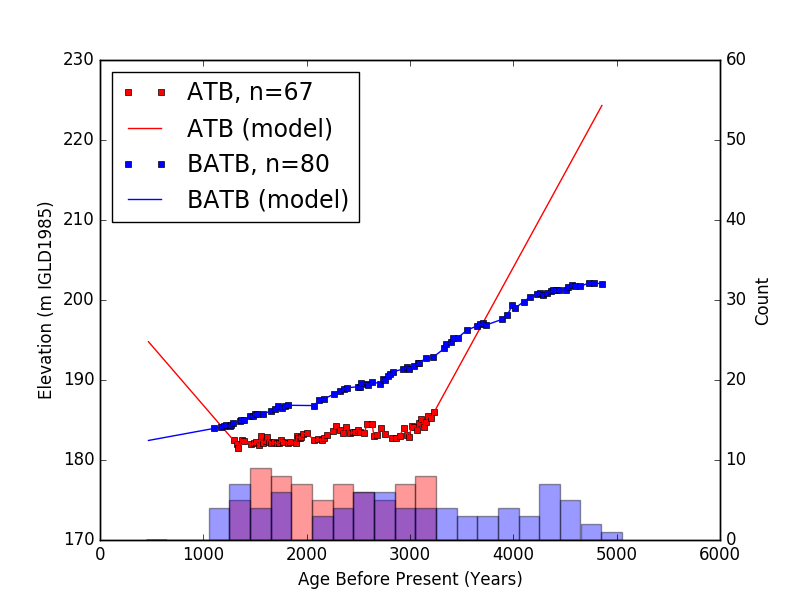
\includegraphics[width=0.72\paperwidth]{data/ATB-BATB_DataAndModel.png}}
	\caption{Measured and modelled elevation data plotted against age for sites ATB \& BATB. Data grouped into bins with widths of 200 years starting at 450 years before present. Bin Counts shown as a histogram at bottom of graph. Histogram bins where both sites overlap are rendered in purple.}
	\label{fig:data_ATBxBATB}
\end{figure}
 Data is available for both ATB and BATB from
 approximately 1000 to 3300 years before present,
 with a gap in the record at around 2000 years before present. With the data divided up into bins of 200 years width
 starting at 450 years before present, the data from every bin between 1250 and 3250 was used
 in calculating a rate of GIA, save for the gap from 1850-2050 years before
 present. The regressions derived from comparing ATB \& BATB are shown
 in Figures \ref{fig:gias_ATBxBATB} \& \ref{fig:gias_BATBxATB}. The GIA rates produced
  indicate that the relative rate of GIA between BATB and ATB of
 between of 24.7 - 31.0 cm/century (ie, BATB rising faster than ATB by this amount). In order to produce this range, a
 regression was done on the differences from both ATB measured data to modelled
 BATB data and vice versa, the results of which are reported in
 the table under Figure \ref{fig:ATBxBATB_regression}. The relative rate of GIA was determined from the
 value of the slopes of each regression, reported here as a 95\% confidence interval
 in cm/century. Once these 95\% intervals were created, a final value was created
 from the range where both confidence intervals overlapped. (for example, with this
 site the two ranges are -24.71 to -31.01 and 23.51 to 31.45 cm/century. Converting
 to absolute value, the overlap between (24.71,31.01) \& (23.51,31.45) is the range
 (24.71,31.01) ). A complete plot of the confidence intervals
 for the slopes obtained from every linear regression done in this paper can be seen in Figure \ref{fig:intervalsGIA}. \\


\begin{figure}[H]
	\begin{flushleft}
	\csvautotabular[respect all]{data/ATB-BATB_regressionTable_bothNonZero_withinSeventyFivePercent.csv}
	\end{flushleft}
	\caption{ATB-BATB Linear regression output parameters. All values reported in cm/century.}
	\label{fig:ATBxBATB_regression}
\end{figure}

\newpage

\begin{figure}[H]
	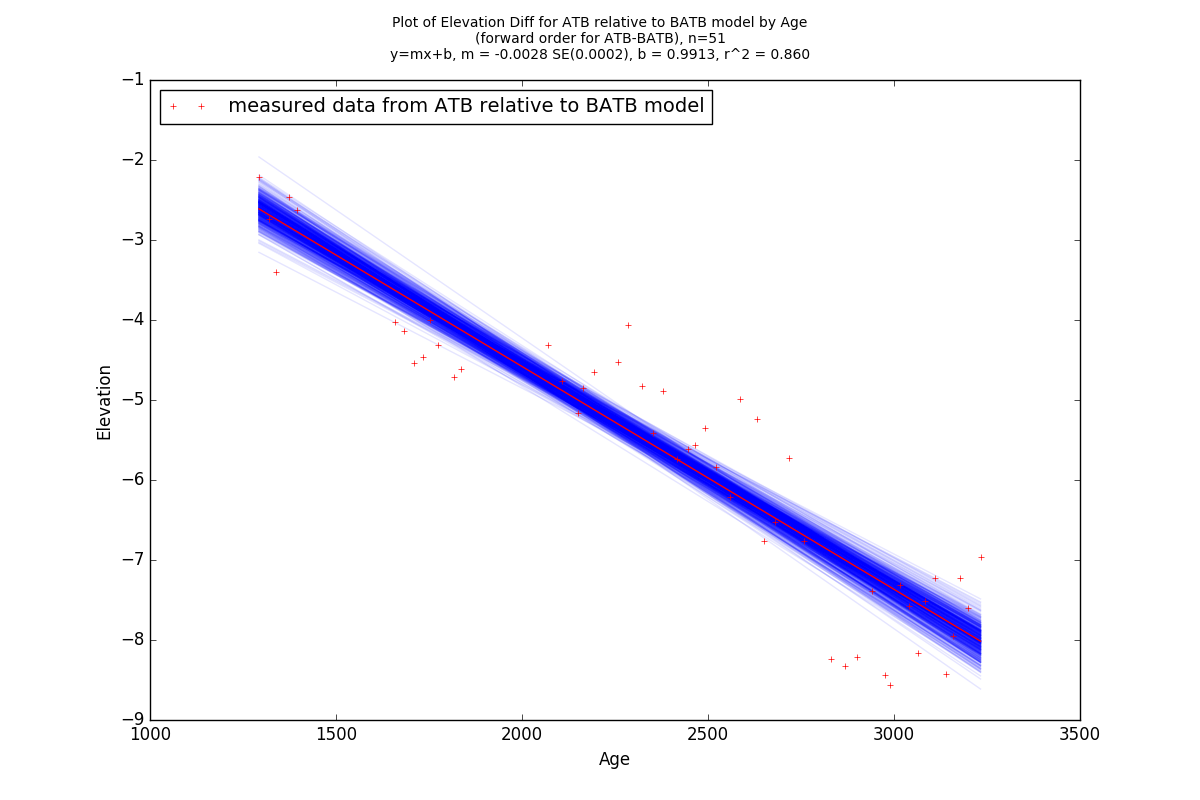
\includegraphics[width=1.3\linewidth, angle=270 ]{data/bothNonZero/withinSeventyFivePercent/gias/theGIA_ATB_relative_to_BATB.png}
	\caption{Plot of differences in elevation from ATB measured data to BATB modelled data. A linear regression with its estimator rendered as
	 a solid red line was fitted to the differences, and a bootstrap for this regression at 95 \% confidence level was rendered in blue
	 around the estimator line.}
	\label{fig:gias_ATBxBATB}
\end{figure}


\begin{figure}[H]
	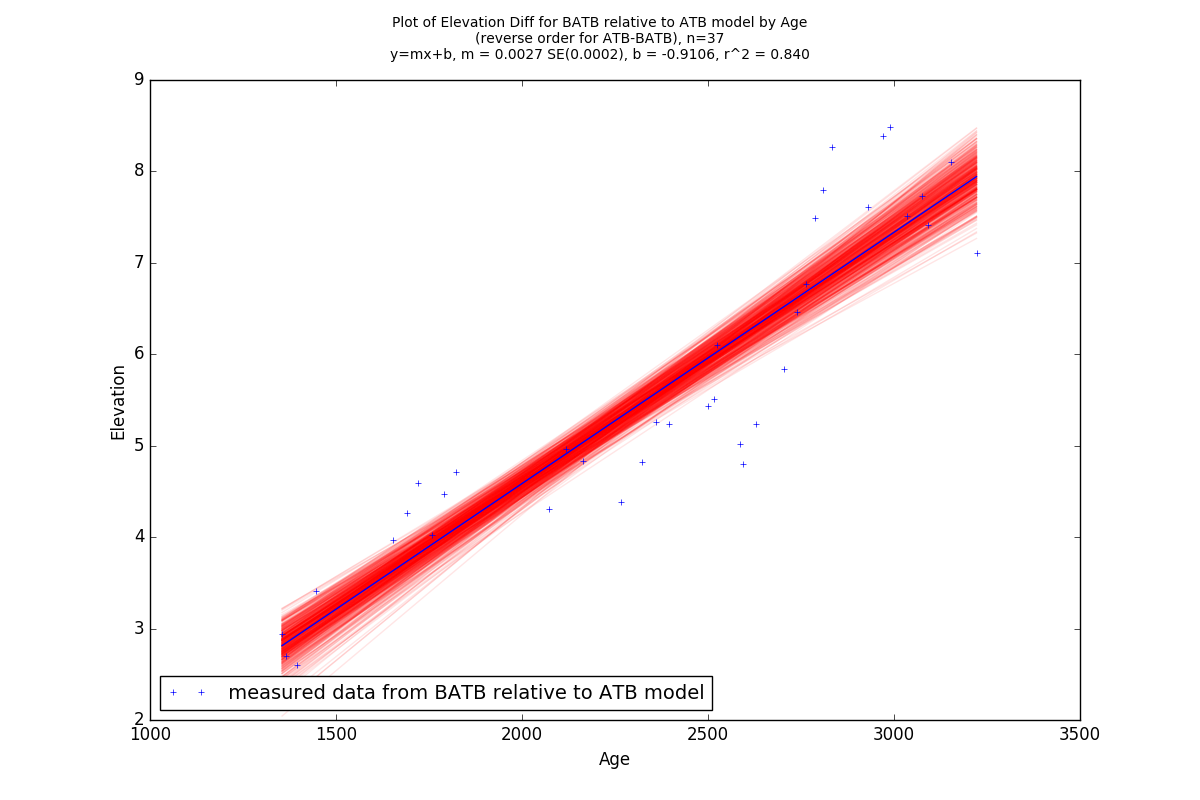
\includegraphics[width=1.3\linewidth, angle=270 ]{data/bothNonZero/withinSeventyFivePercent/gias/theGIA_BATB_relative_to_ATB.png}
	\caption{Plot of differences in elevation from BATB measured data to ATB modelled data. A linear regression with its estimator rendered as
	 a solid blue line was fitted to the differences, and a bootstrap for this regression at 95 \% confidence level was rendered in red
	 around the estimator line.}
	\label{fig:gias_BATBxATB}
\end{figure}
\newpage
% this desperately needs to be done as a loop













\subsubsection{TAHB-BATB}

\begin{figure}[H]
	\makebox[\textwidth]{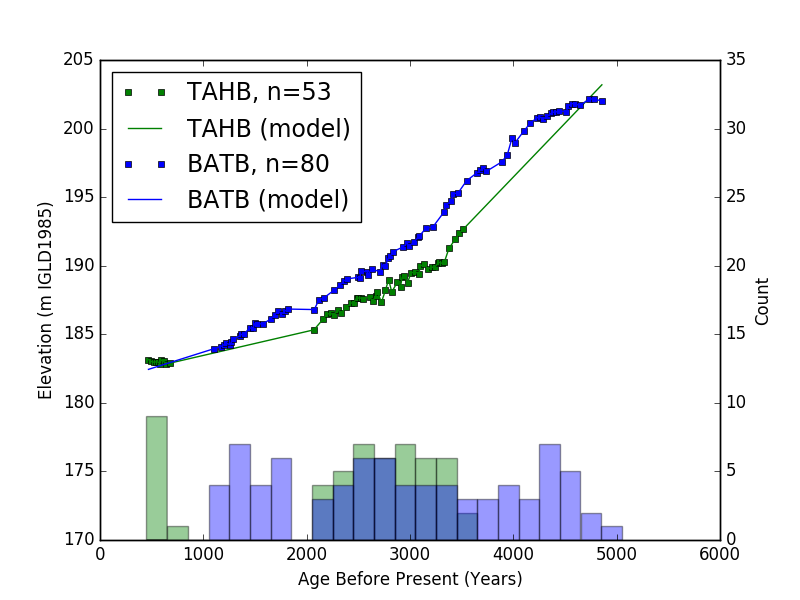
\includegraphics[width=0.72\paperwidth]{data/TAHB-BATB_DataAndModel.png}}
	\caption{Measured and modelled elevation data plotted against age for sites TAHB \& BATB. Data grouped into bins with widths of 200 years starting at 450 years before present. Bin Counts shown as a histogram at bottom of graph.}	
	\label{fig:data_TAHBxBATB}
\end{figure}

The data plot for the site combination of TAHB and BATB used a filter which 
grouped data points into bins 200 years wide starting at 450 years before present,
ignoring the data points from bins in which either data set had no datapoints,
as well as any which had bin counts differing by more than 75\% for that bin.
As a result, only the data from 2050 to 3650 years before present were used in
creating the GIA comparisons between TAHB and BATB.\\
The linear regressions produced from this pair of datasets are shown in Figures 
\ref{fig:gias_TAHBxBATB} \& \ref{fig:gias_BATBxTAHB}, with the parameters for each
regression listed in Figure \ref{fig:TAHBxBATB_regression}. Merging the two ranges
reported under the "Slope C.I. (95p)" column in Figure \ref{fig:TAHBxBATB_regression} gave
a value for relative GIA of between 11.9-16.8 cm/century. \\


\begin{figure}[H]
	\begin{flushleft}
	\csvautotabular[respect all]{data/TAHB-BATB_regressionTable_bothNonZero_withinSeventyFivePercent.csv}
	\end{flushleft}
	\caption{TAHB-BATB Regression output parameters. All values reported in cm/century.}
	\label{fig:TAHBxBATB_regression}
\end{figure}


\newpage

\begin{figure}[H]
	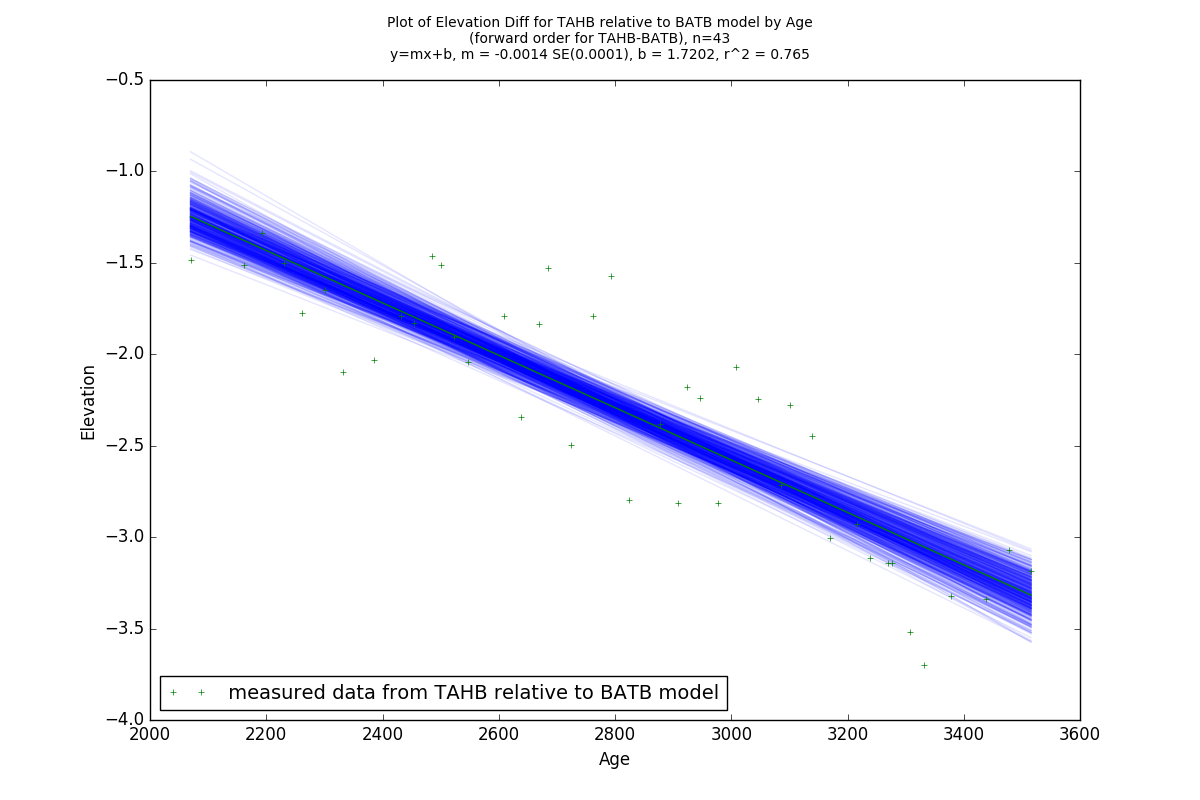
\includegraphics[width=1.3\linewidth, angle=270 ]{data/bothNonZero/withinSeventyFivePercent/gias/theGIA_TAHB_relative_to_BATB.png}
	\caption{Plot of differences in elevation from TAHB measured data to BATB modelled data. A linear regression with its estimator rendered as
	 a solid green line was fitted to the differences, and a bootstrap for this regression at 95 \% confidence level was rendered in blue
	 around the estimator line.}
	\label{fig:gias_TAHBxBATB}
\end{figure}
\newpage


\begin{figure}[H]
	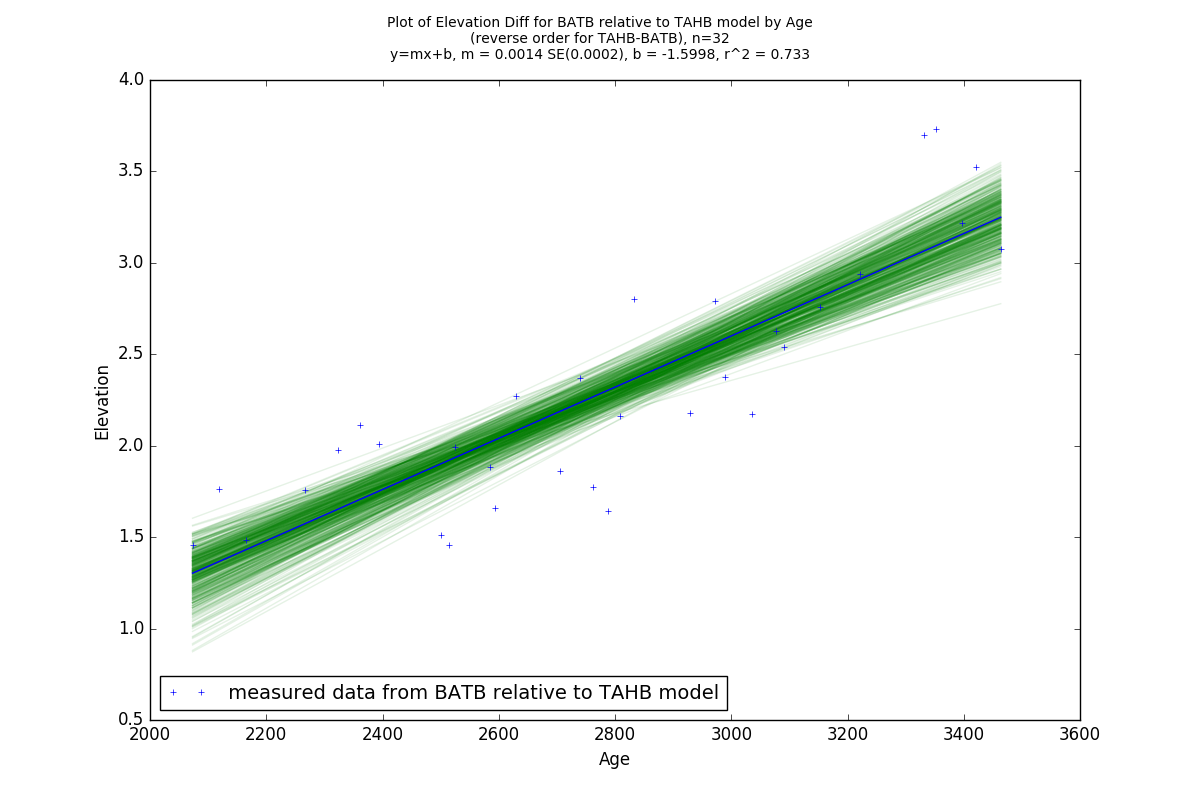
\includegraphics[width=1.3\linewidth, angle=270 ]{data/bothNonZero/withinSeventyFivePercent/gias/theGIA_BATB_relative_to_TAHB.png}
	\caption{Plot of differences in elevation from BATB measured data to TAHB modelled data. A linear regression with its estimator rendered as
	 a solid blue line was fitted to the differences, and a bootstrap for this regression at 95 \% confidence level was rendered in green
	 around the estimator line.}
	\label{fig:gias_BATBxTAHB}
\end{figure}
\newpage






\subsubsection{TAHB-ATB}

\begin{figure}[H]
	\makebox[\textwidth]{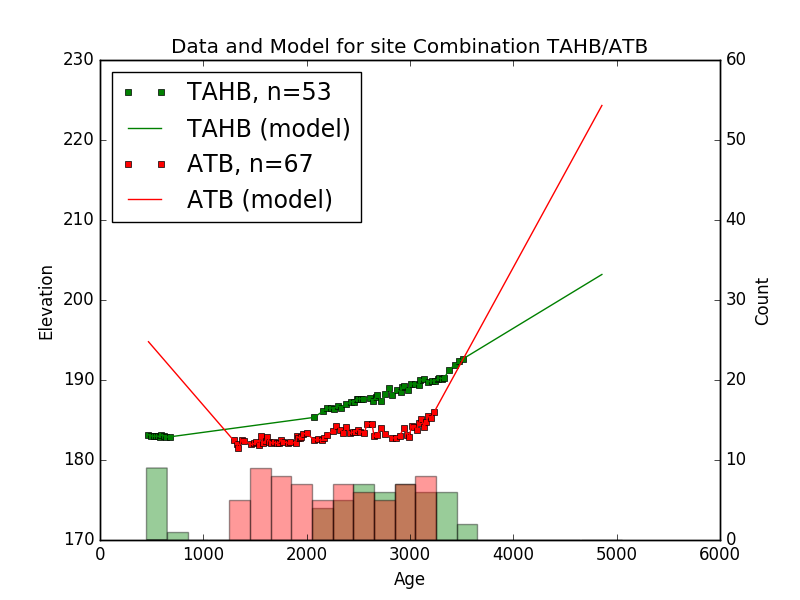
\includegraphics[width=0.72\paperwidth]{data/TAHB-ATB_DataAndModel.png}}
	\caption{Measured and modelled elevation data plotted against age for sites TAHB \& ATB. Data grouped into bins with widths of 200 years starting at 450 years before present. Bin Counts shown as a histogram at bottom of graph.}	
	\label{fig:data_TAHBxATB}
\end{figure}

Similar to previous dataset comparisons TAHB-BATB and ATB-BATB, the combination of TAHB and ATB are constrained to
ages older than
2050 years before present, but also have a much shorter range
of age values that
can be considered for GIA calculation, starting at 2000 and ending at around 3100 years before present.
As a result, only datapoints between 2050 and 3250 years before present
were used, resulting in
relatively poor regressions ($R^2$ values close to 0.5 where TAHB-BATB and ATB-BATB
were both well above 0.7) reported in Figure \ref{fig:TAHBxATB_regression}.
The weak correlation of these regressions results in a wide range for
relative GIA of between 19.4-29.2 cm/century. \\


\begin{figure}[H]
	\begin{flushleft}
	\csvautotabular[respect all]{data/TAHB-ATB_regressionTable_bothNonZero_withinSeventyFivePercent.csv}
	\end{flushleft}
	\caption{TAHB-ATB Regression output parameters. All values reported in cm/century.}
	\label{fig:TAHBxATB_regression}
\end{figure}


\newpage

\begin{figure}[H]
	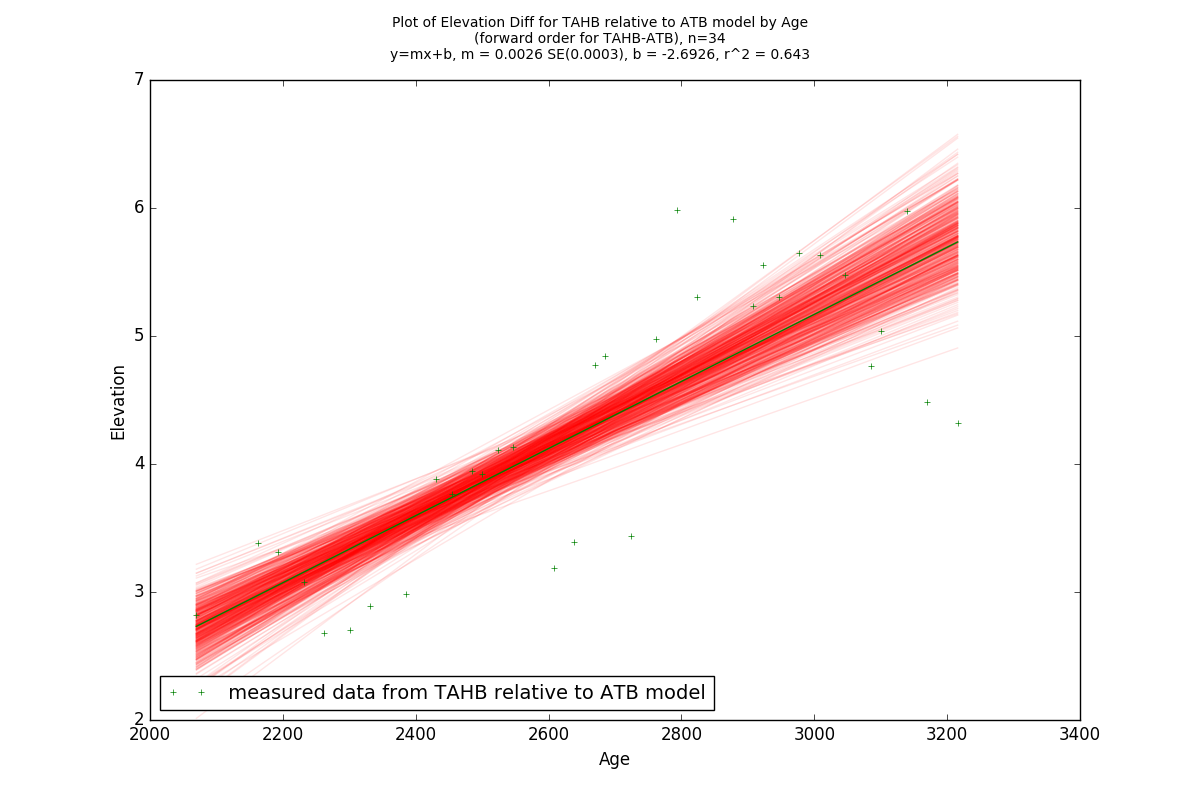
\includegraphics[width=1.3\linewidth, angle=270 ]{data/bothNonZero/withinSeventyFivePercent/gias/theGIA_TAHB_relative_to_ATB.png}
	\caption{Plot of differences in elevation from TAHB measured data to ATB modelled data. A linear regression with its estimator rendered as
	 a solid green line was fitted to the differences, and a bootstrap for this regression at 95 \% confidence level was rendered in red
	 around the estimator line.}
	\label{fig:gias_TAHBxATB}
\end{figure}
\newpage


\begin{figure}[H]
	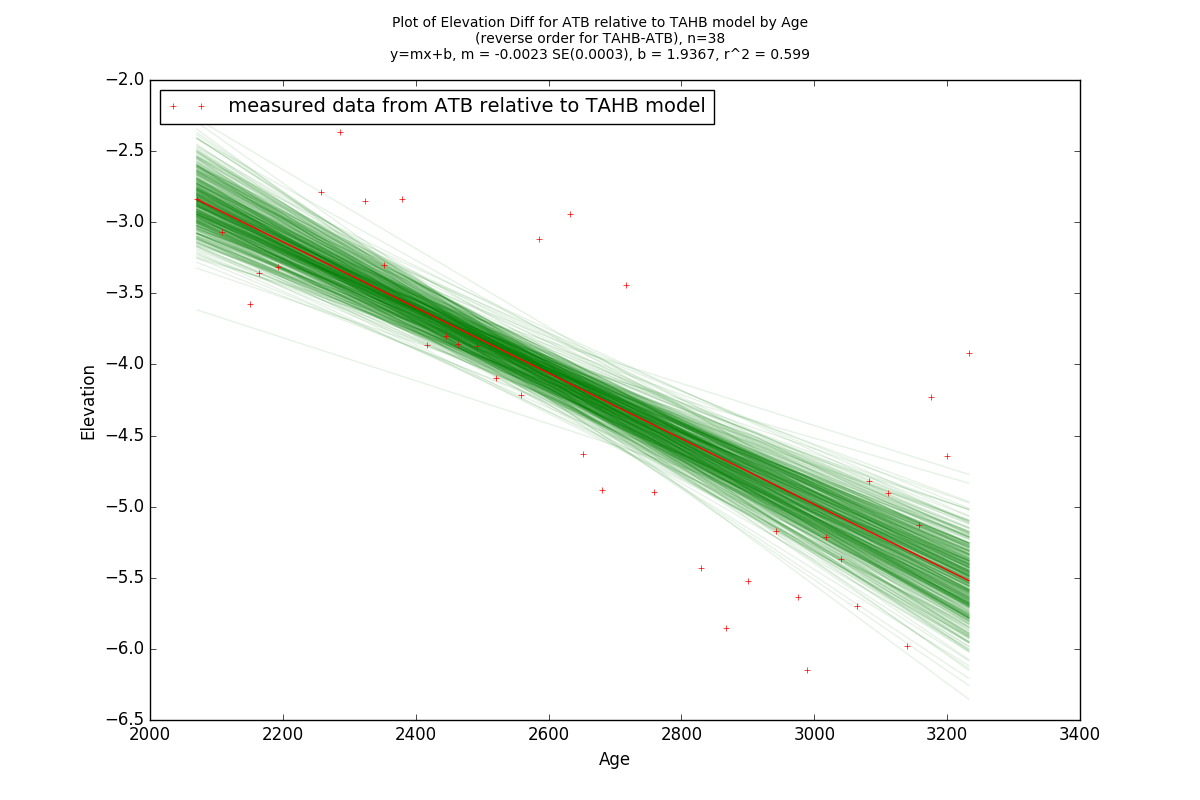
\includegraphics[width=1.3\linewidth, angle=270 ]{data/bothNonZero/withinSeventyFivePercent/gias/theGIA_ATB_relative_to_TAHB.png}
	\caption{Plot of differences in elevation from ATB measured data to TAHB modelled data. A linear regression with its estimator rendered as
	 a solid red line was fitted to the differences, and a bootstrap for this regression at 95 \% confidence level was rendered in green
	 around the estimator line.}
	\label{fig:gias_ATBxTAHB}
\end{figure}
\newpage




\subsubsection{GTB-BATB}

\begin{figure}[H]
	\makebox[\textwidth]{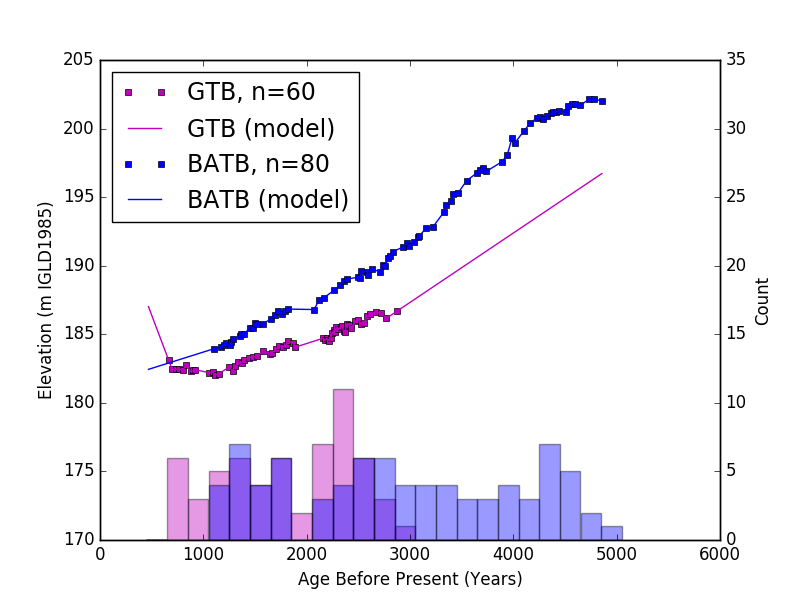
\includegraphics[width=0.72\paperwidth]{data/GTB-BATB_DataAndModel.png}}
	\caption{Measured and modelled elevation data plotted against age for sites GTB \& BATB. Data grouped into bins with widths of 200 years starting at 450 years before present. Bin Counts shown as a histogram at bottom of graph.}	
	\label{fig:data_GTBxBATB}
\end{figure}
The GTB BATB combination has data available for both datasets from 1050 to 3050 years before present with 
a gap in coverage from 1850 to 2050 years before present. The first case of the
75\% difference cutoff rule for bin inclusion has its first appearance here as
only the oldest shoreline available from GTB falls inside of the 2850-3050 years
before present window, causing the entire window to be
used if the only criteria was both dataset counts within that window being non-zero.
The 75\% cutoff prevents this window from being used in this case, as the counts
for the bin at 2850-3050 years before present differ by 120\% between GTB and BATB. This rule is useful in identifying
areas of the dataset where both sites have data available, but the density of
one of the datasets in that region is low enough to potentially cause inaccurate
predictions where modelled elevation extends a long distance between measured datapoints.
The regressions plotted in
Figures \ref{fig:gias_GTBxBATB} \& \ref{fig:gias_BATBxGTB} are listed in 
Figure \ref{fig:GTBxBATB_regression}. The $R^2$ values for both regressions
are well over 0.8, and the ranges for relative GIA listed under the "Slope C.I. (95p)" column
agree to within less than 1 cm/century,
producing one of the most well constrained values seen in this paper at 10.5-13.4 cm/century. \\


\begin{figure}[H]
	\begin{flushleft}
	\csvautotabular[respect all]{data/GTB-BATB_regressionTable_bothNonZero_withinSeventyFivePercent.csv}
	\end{flushleft}
	\caption{GTB-BATB Regression output parameters. All values reported in cm/century.}
	\label{fig:GTBxBATB_regression}
\end{figure}

\newpage

\begin{figure}[H]
	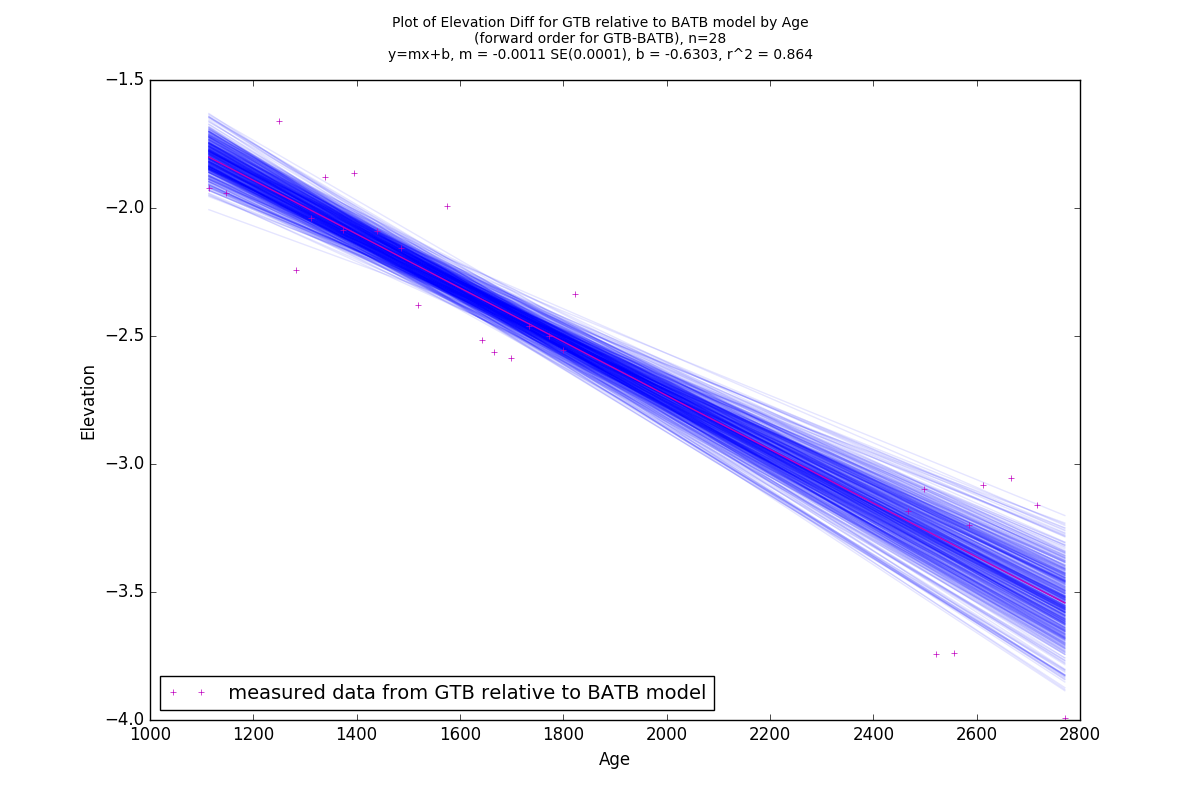
\includegraphics[width=1.3\linewidth, angle=270 ]{data/bothNonZero/withinSeventyFivePercent/gias/theGIA_GTB_relative_to_BATB.png}
	\caption{Plot of differences in elevation from GTB measured data to BATB modelled data. A linear regression with its estimator rendered as
	 a solid purple line was fitted to the differences, and a bootstrap for this regression at 95 \% confidence level was rendered in blue
	 around the estimator line.}
	\label{fig:gias_GTBxBATB}
\end{figure}
\newpage


\begin{figure}[H]
	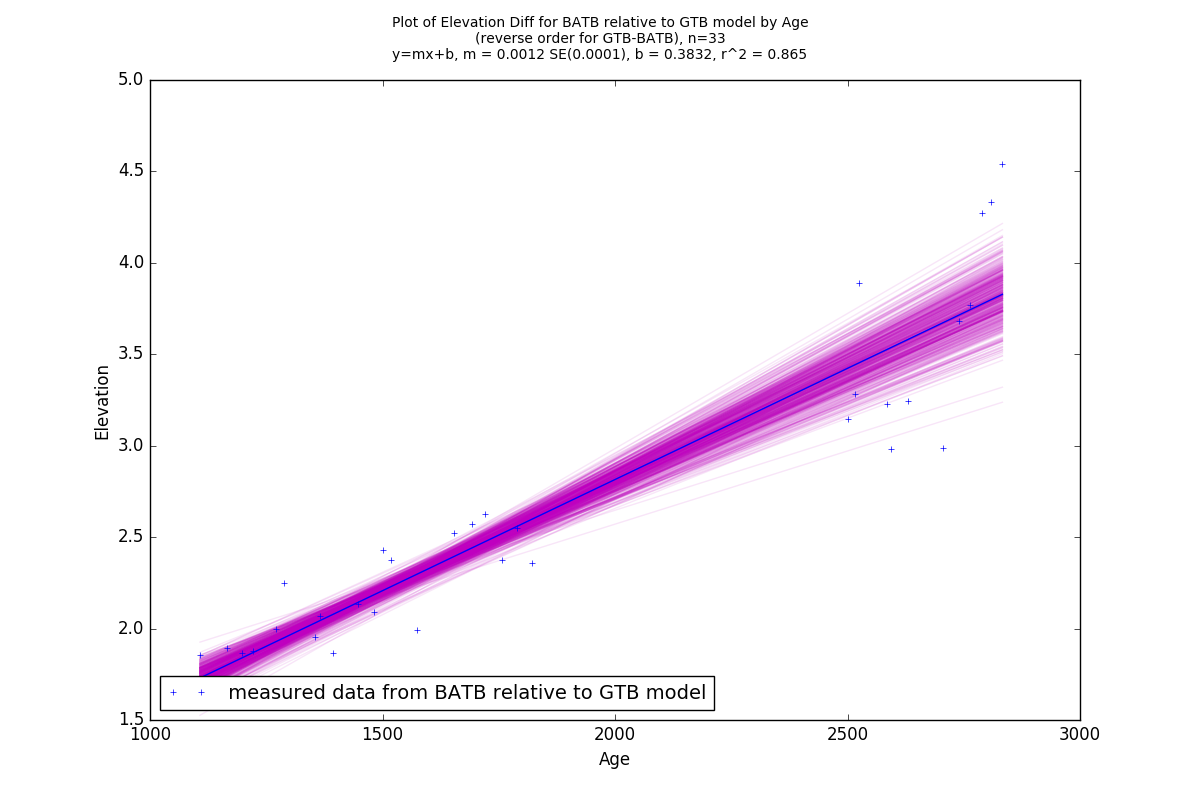
\includegraphics[width=1.3\linewidth, angle=270 ]{data/bothNonZero/withinSeventyFivePercent/gias/theGIA_BATB_relative_to_GTB.png}
	\caption{Plot of differences in elevation from BATB measured data to GTB modelled data. A linear regression with its estimator rendered as
	 a solid blue line was fitted to the differences, and a bootstrap for this regression at 95 \% confidence level was rendered in purple
	 around the estimator line.}
	\label{fig:gias_BATBxGTB}
\end{figure}
\newpage







\subsubsection{GTB-ATB}

\begin{figure}[H]
	\makebox[\textwidth]{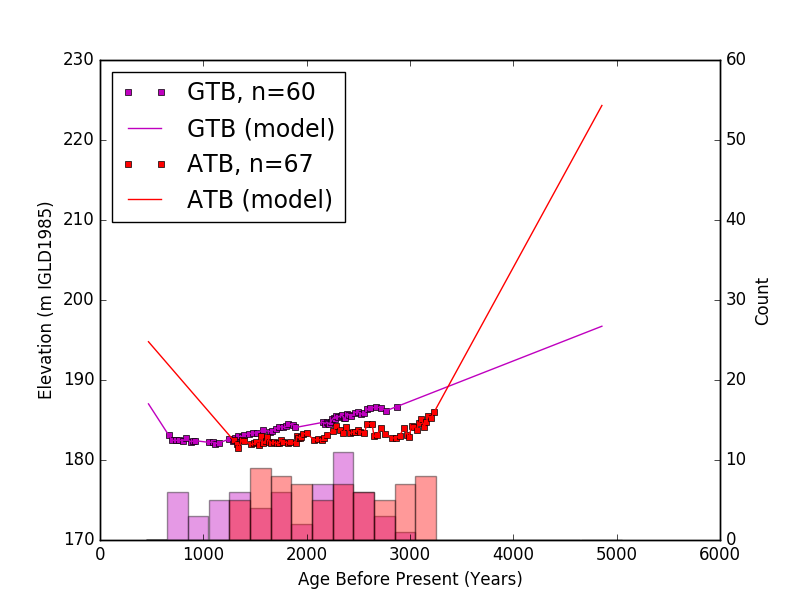
\includegraphics[width=0.72\paperwidth]{data/GTB-ATB_DataAndModel.png}}
	\caption{Measured and modelled elevation data plotted against age for sites GTB \& ATB. Data grouped into bins with widths of 200 years starting at 450 years before present. Bin Counts shown as a histogram at bottom of graph.}	
	\label{fig:data_GTBxATB}
\end{figure}

The GTB-ATB combination has
bins from 1250 to 3050 years before present containing data for both sites. Two of these bins
fail to qualify for use due to the site counts differing by more
than 75\%. These bins can be seen at 1850-2050, and 2850 to 3050 years before present. 
In Figure \ref{fig:data_GTBxATB}, it can be seen that both of these bins coincide with ranges of
time where GTB has sparse data, making the GTB models predictions unreliable in that bin.
The regressions plotted in Figures \ref{fig:gias_GTBxATB} \& \ref{fig:gias_ATBxGTB}, and
listed in Figure \ref{fig:GTBxATB_regression}. These regressions have weak correlations
(with $R^2$ values of 0.427 and 0.595 respectively), and only overlap in a small
range of 10.5-13.5 cm/century. Although this range appears very precise, the measurement
is likely inaccurate, as the comparisons do not agree very well between the forward
and reverse comparisons, the ranges of GIA produced from each regression only
overlapping for a small fraction of their respective ranges at the 95\% confidence
level.\\

\begin{figure}[H]
	\begin{flushleft}
	\csvautotabular[respect all]{data/GTB-ATB_regressionTable_bothNonZero_withinSeventyFivePercent.csv}
	\end{flushleft}
	\caption{GTB-ATB Regression output parameters. All values reported in cm/century.}
	\label{fig:GTBxATB_regression}
\end{figure}

\newpage

\begin{figure}[H]
	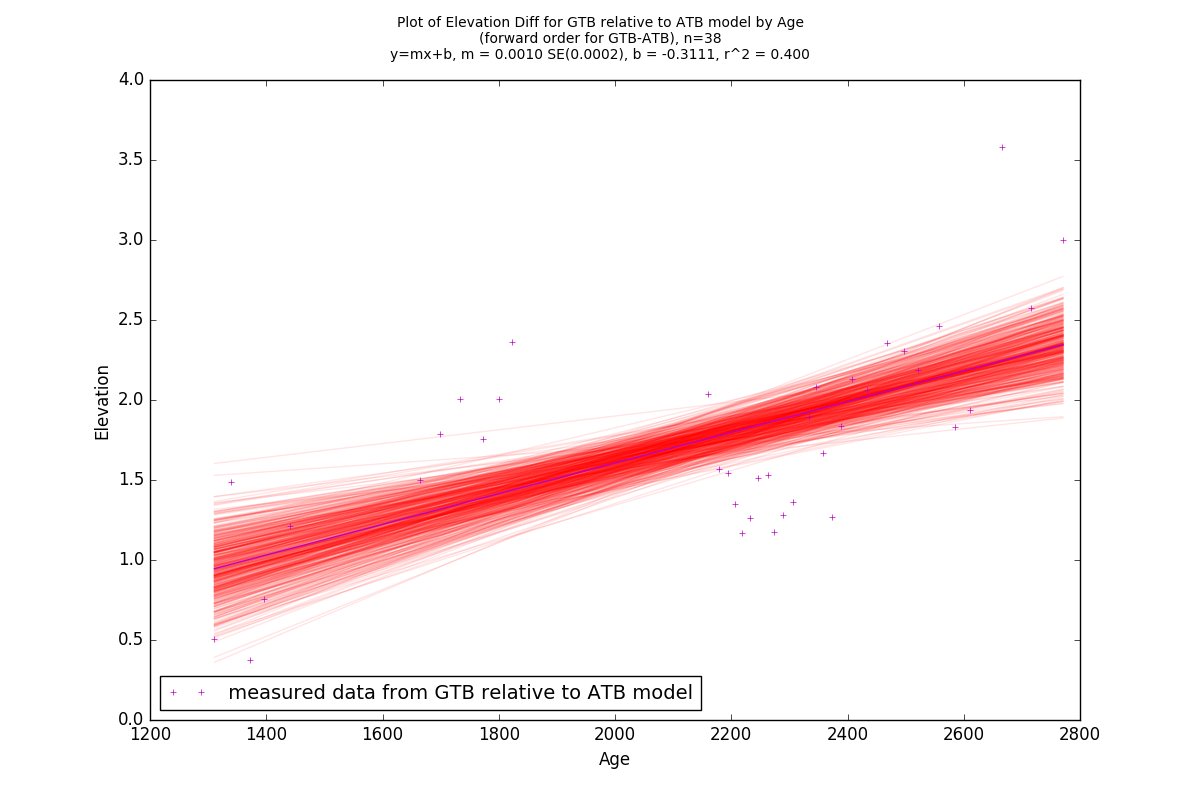
\includegraphics[width=1.3\linewidth, angle=270 ]{data/bothNonZero/withinSeventyFivePercent/gias/theGIA_GTB_relative_to_ATB.png}
	\caption{Plot of differences in elevation from GTB measured data to ATB modelled data. A linear regression with its estimator rendered as
	 a solid purple line was fitted to the differences, and a bootstrap for this regression at 95 \% confidence level was rendered in red
	 around the estimator line.}
	\label{fig:gias_GTBxATB}
\end{figure}
\newpage


\begin{figure}[H]
	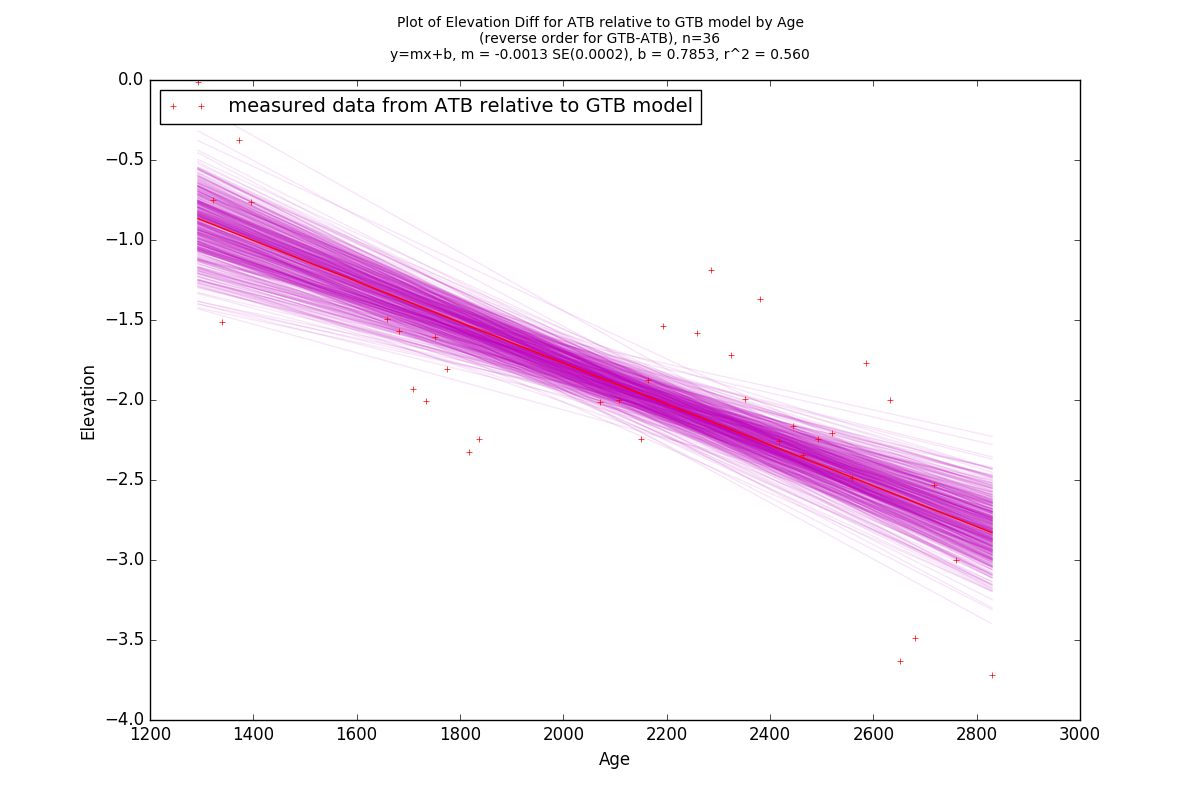
\includegraphics[width=1.3\linewidth, angle=270 ]{data/bothNonZero/withinSeventyFivePercent/gias/theGIA_ATB_relative_to_GTB.png}
	\caption{Plot of differences in elevation from ATB measured data to GTB modelled data. A linear regression with its estimator rendered as
	 a solid red line was fitted to the differences, and a bootstrap for this regression at 95 \% confidence level was rendered in purple
	 around the estimator line.}
	\label{fig:gias_ATBxGTB}
\end{figure}
\newpage








\subsubsection{GTB-TAHB}

\begin{figure}[H]
	\makebox[\textwidth]{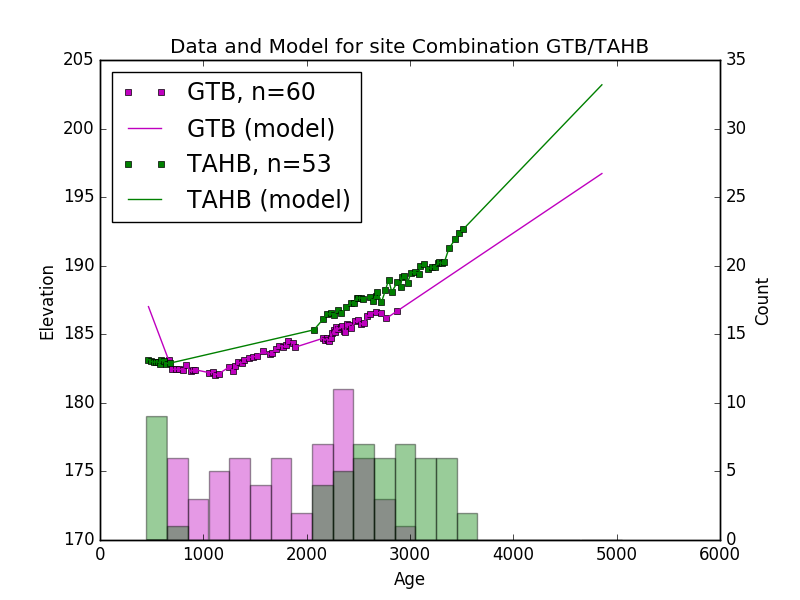
\includegraphics[width=0.72\paperwidth]{data/GTB-TAHB_DataAndModel.png}}
	\caption{Measured and modelled elevation data plotted against age for sites GTB \& TAHB. Data grouped into bins with widths of 200 years starting at 450 years before present. Bin Counts shown as a histogram at bottom of graph.}	
	\label{fig:data_GTBxTAHB}
\end{figure}
The combination of sites GTB and TAHB has data in bins from 450 to 3650 years before
present, of which only 2050 to 2850 years before present was used. Two
potential bins located at 650-850 and 2850-3050 years before present were not used due failing to
meet the 75\% rule, both would have produced comparisons between areas of
data in one dataset and a poorly constrained model in the other.

The combination of sites GTB and TAHB has by far the poorest regressions, listed
in \ref{fig:GTBxTAHB_regression}. This is likely due to the alignment of most
of both datasets only giving limited sample sizes of n=22 (Figure \ref{fig:gias_TAHBxGTB})
and n=27 (Figure \ref{fig:gias_GTBxTAHB}) for comparisons. 
This resulted in an estimate of GIA that ranges anywhere from -2.8-8.6 cm/century,
possibly implying that the relative difference in vertical adjustment rates
between the TAHB and GTB sites may be zero. \\

\begin{figure}[H]
	\begin{flushleft}
	\csvautotabular[respect all]{data/GTB-TAHB_regressionTable_bothNonZero_withinSeventyFivePercent.csv}
	\end{flushleft}
	\caption{GTB-TAHB Regression output parameters. All values reported in cm/century.}
	\label{fig:GTBxTAHB_regression}
\end{figure}

\newpage

\begin{figure}[H]
	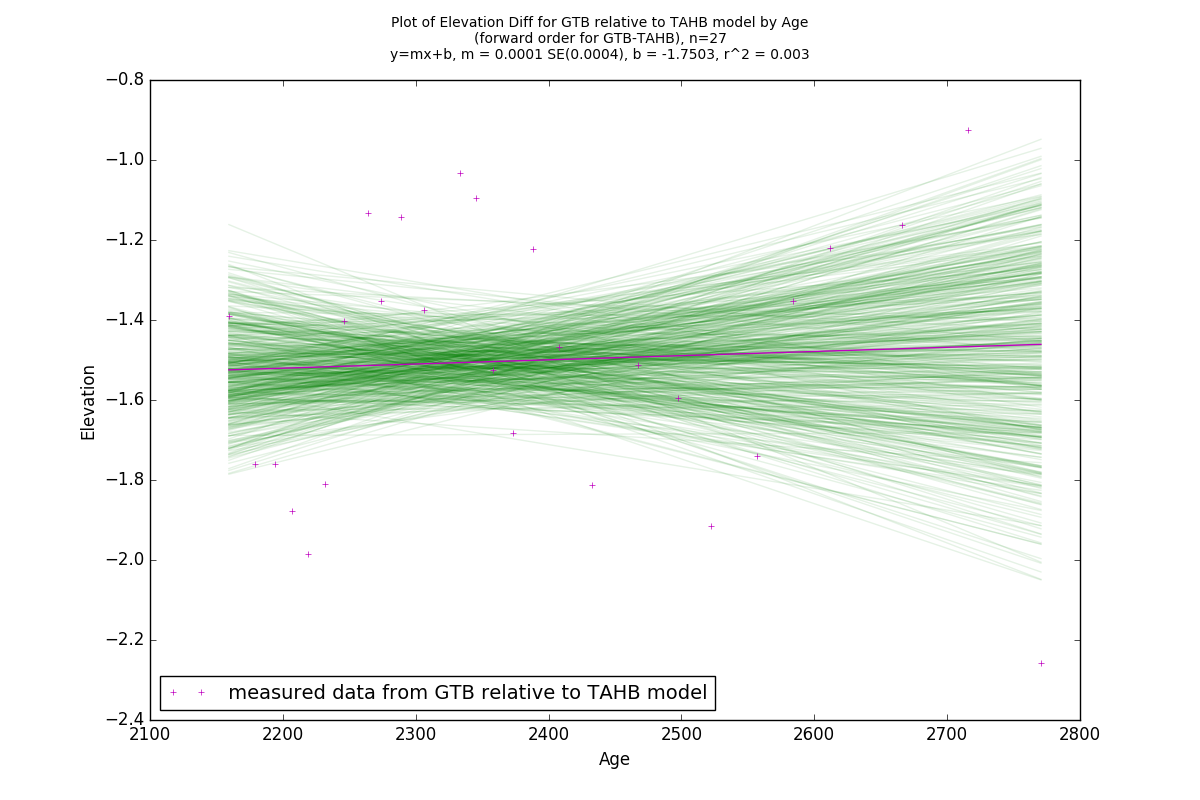
\includegraphics[width=1.3\linewidth, angle=270 ]{data/bothNonZero/withinSeventyFivePercent/gias/theGIA_GTB_relative_to_TAHB.png}
	\caption{Plot of differences in elevation from ATB measured data to GTB modelled data. A linear regression with its estimator rendered as
	 a solid purple line was fitted to the differences, and a bootstrap for this regression at 95 \% confidence level was rendered in green
	 around the estimator line.}
	\label{fig:gias_GTBxTAHB}
\end{figure}
\newpage


\begin{figure}[H]
	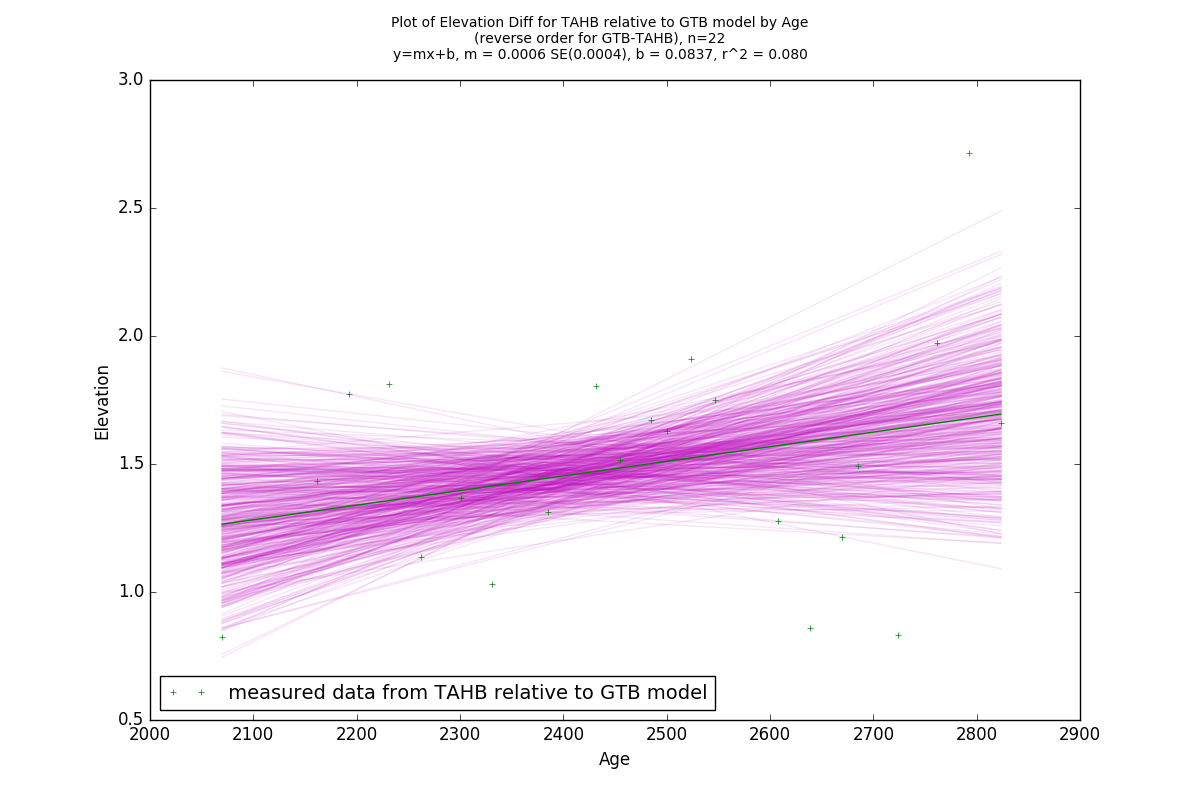
\includegraphics[width=1.3\linewidth, angle=270 ]{data/bothNonZero/withinSeventyFivePercent/gias/theGIA_TAHB_relative_to_GTB.png}
	\caption{Plot of differences in elevation from GTB measured data to ATB modelled data. A linear regression with its estimator rendered as
	 a solid green line was fitted to the differences, and a bootstrap for this regression at 95 \% confidence level was rendered in purple
	 around the estimator line.}
	\label{fig:gias_TAHBxGTB}
\end{figure}
\newpage

\subsubsection{Summary of calculated GIA values}

\begin{figure}[H]
	\makebox[\textwidth]{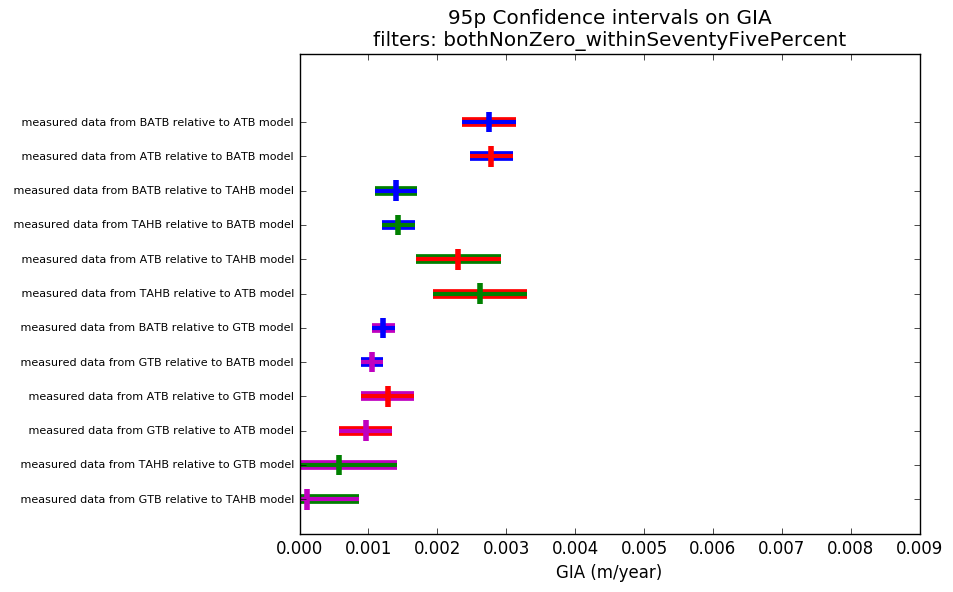
\includegraphics[width=0.6\paperwidth]{data/bothNonZero/withinSeventyFivePercent/gias/intervals.png}}
	\caption{Confidence intervals at the 95 \% confidence level for relative GIA rates obtained from 12 intra-site comparisons across 4 sites.}
	\label{fig:intervalsGIA}
\end{figure}


\newpage

